\section{The Live Gap}
\label{sec:livegap}

The first deployment (the \emph{shipped build}) ran the v1 CNN behind a browser pipeline that
computed the same named features as training but not always the same values, and it recognized
almost nothing live. We audited six candidate train--serve discrepancies between that pipeline and
the training preprocessing, fixed each so that the browser reproduces Python
(Figure~\ref{fig:pipeline}), and measured each fix on new recordings. Not every candidate turned out
to be a fault of the shipped build; for each we state what it did.

\begin{figure}[t]
\centering
\begin{tikzpicture}[
  node distance=1.6mm and 2.6mm,
  box/.style={draw=black!55, rounded corners=1.5pt, fill=black!4, align=center, font=\scriptsize,
              inner sep=2.2pt, minimum height=6.5mm},
  live/.style={box, fill=orange!12, draw=orange!70!black},
  arr/.style={-{Stealth[length=1.6mm]}, black!70, line width=0.45pt}]
  \node[box] (cam) {Webcam\\frame};
  \node[box, right=of cam] (mp) {MediaPipe Tasks\\hands + pose\\(worker 1)};
  \node[live, right=of mp] (map) {Holistic layout\\(a) hands, (b) unmirrored,\\(c) aspect};
  \node[live, below=of map] (seg) {Segmenter (e)\\time resampling (d)};
  \node[box, left=of seg] (cls) {Hybrid fp16\\onnxruntime-web\\(worker 2)};
  \node[live, left=of cls] (dec) {Temperature +\\threshold (f)};
  \node[box, below=of dec, xshift=6mm] (out) {Gloss row or\\``not sure''};
  \draw[arr] (cam) -- (mp);
  \draw[arr] (mp) -- (map);
  \draw[arr] (map) -- (seg);
  \draw[arr] (seg) -- (cls);
  \draw[arr] (cls) -- (dec);
  \draw[arr] (dec.south) -- (dec.south |- out.north);
\end{tikzpicture}
\caption{The live pipeline in the browser. Orange boxes are the six audited steps; each reads its
constants from \cfg{features\_spec.json} or the model metadata, which the Python training code also
reads.}
\label{fig:pipeline}
\end{figure}

\subsection{Six candidate discrepancies}
\label{sec:faults}

\paragraph{(a) Hand slots.} Holistic, which produced the training data, crops each hand from the
pose, so its \emph{left hand} block is the hand at the signer's left wrist. The browser's
HandLandmarker reports a handedness label instead, and the shipped build mapped that label as if
the frame were mirrored while it ran detection on the unmirrored frame, so every hand went into the
wrong block. The fix assigns each detected hand to the block of the nearer pose wrist, Holistic's
own rule, and falls back to the label only when there is no pose.

\paragraph{(b) Mirroring.} The shipped build already detected landmarks on the unmirrored frame;
we test detection on the mirrored frame, as a selfie pipeline would do it, as a counterfactual.

\paragraph{(c) Aspect ratio.} Coordinates are normalized by the image width and height, so the
same body has different normalized proportions in a portrait phone recording and a wide webcam.
The shipped build corrected for this with a body-ratio estimate over the first two seconds. The fix
replaces it by a rule from the frame size: we estimate the training data's width-to-height ratio
from face geometry on the training split (\V{asp.train}) and rescale live y coordinates about the
shoulder midpoint by $k = r_{\mathrm{train}} / (w/h)$, with the real width and height of the frame.

\paragraph{(d) Frame rate.} Training resampled each sequence to \V{data.frames} frames by frame
index; the dataset has no timestamps. The browser's frame rate varies with the camera and the load,
so resampling by index stretches or compresses time; the fix resamples on the capture-time clock.

\paragraph{(e) Segmentation.} The shipped build segmented by hand presence: a segment starts after
\V{pres.start} frames with a hand and ends after \V{pres.end} without one or after \V{pres.max} s.
The fix is a state machine on motion energy, the speed of the wrist and fingertips in shoulder
widths per second on aspect-corrected coordinates, so (c) and (e) interact. A sign starts when a
hand is present and the energy exceeds \V{seg.start}, and ends when the hands are lost for
\V{seg.lostms} ms, stay below \V{seg.still} for \V{seg.stillms} ms, or after \V{seg.maxs} s;
segments shorter than \V{seg.minms} ms are discarded, and gaps up to \V{seg.gapms} ms are bridged.
The thresholds come from the validation sequences, assuming their frames are \V{seg.assumedfps} fps
apart: the start threshold is the \V{seg.startpct}th percentile of the per-sequence peak energy, and
the still threshold the largest value at which at most \V{seg.stillpct}\% of sequences would be cut
inside the sign.

\paragraph{(f) Calibration and abstention.} The shipped build showed the raw top-1 above a
threshold set for \V{cal.targetprec}\% precision on validation. The fix divides the logits by a
temperature fitted on validation (\V{cal.T}) and shows a word only if its probability reaches a
threshold chosen on validation to maximize the net score, coverage times twice the selective
accuracy minus one, so a correct accepted word gains one, a wrong one costs one and ``not sure''
scores zero \citep{guo2017calibration,geifman2017selective}.

\paragraph{One specification, one test.} The landmark subset, normalization, mirroring,
resampling, aspect constant and segmenter thresholds live in \cfg{features\_spec.json}, which
Python and the browser both read. A golden-fixture test runs the browser code on the raw landmarks
of \V{par.cases} validation sequences, exported from Python with Python's features and logits, and
requires every model input to match within \V{par.tol} and the top-1 class to agree; it covers hand
assignment and replays a stream through the segmenter frame by frame. It runs in continuous
integration, so a change to either implementation that alters a feature fails the build.

\subsection{Evaluation on new recordings}

\paragraph{Clips.} The author recorded \V{lg.clips} clips with a laptop webcam: \V{lg.signs}
signs from the vocabulary (\authortodo{how the signs were chosen, and the source of the sign
forms}), two takes each (median \V{lg.duration}\,s), unmirrored at \V{lg.width}$\times$\V{lg.height}
and about \V{lg.fps} frames per second (Figure~\ref{fig:skeleton} in the appendix), scaled to
\V{lg.ywidth}$\times$\V{lg.yheight} for both pipelines. No clip duplicates another. The author is
both the developer and the only signer, and the order of the fixes was motivated by a pilot of the
same person (Appendix~\ref{app:pilot}). Nothing was tuned on these clips: every threshold, the
temperature and the aspect constant come from the training and validation splits, and the analysis
was written into the configuration before the first run.

\paragraph{Pipelines.} \emph{Python + Holistic} runs legacy MediaPipe Holistic, the tracker that
produced the training data, on every frame and then the Python live pipeline; it is deterministic.
\emph{Browser + Tasks} runs the web app in Chrome on the target laptop with the clip as a fake
camera, in real time, so frames are dropped as they would be live. One browser per clip runs every
configuration in a seeded random order, so drift of the laptop does not fall on one configuration;
each configuration runs three times (Table~\ref{tab:livegapci} gives the count per row) and a clip's
score is its mean over the runs. In \V{lg.stalled} of \V{lg.browserrecords} browser records the
tracker processed fewer than half of the clip's frames; they are kept as measured. There are two
baselines: the \emph{shipped build} itself, which
runs MediaPipe and the classifier on the page's main thread at \V{lg.web.c0headbuild.fps}
frames per second, and \emph{as shipped}, the current app with the shipped build's settings at
\V{lg.web.c0asshipped.fps}.

\paragraph{Scoring and statistics.} A clip's prediction is the mean probability vector of its
classified segments; a clip without one counts as wrong. We report clip-level top-1 and top-3 with
percentile bootstrap intervals over clips \citep{efron1994bootstrap}. Each configuration is
compared with the one it modifies by a two-sided paired sign-flip permutation test on per-clip
scores \citep{dror2018hitchhiker}, and the p-values of each pipeline and metric are adjusted with
Holm's step-down procedure \citep{dror2017replicability}; the difference intervals are not adjusted.
This clip-level analysis was specified before the runs. Because the two takes of a sign are not
independent, we add a sensitivity analysis after the fact that treats each sign as one unit. The
families include comparisons that cannot change top-1 by construction, and error rates are
controlled within, not across, families. Power is low: to reach significance at the first Holm
step, at least \V{mde.web.k} clips (\V{mde.web.pts} points) must all move in one direction in the
browser and \V{mde.py.k} in Python, so smaller effects are inconclusive rather than absent
\citep{card2020power}.

\subsection{Results}
\label{sec:liveresults}

% Generated by scripts/paper_tables.py -- do not edit.
\typeout{[table livegap]}
\begin{table}[t]
\centering
\footnotesize
\setlength{\tabcolsep}{3pt}
\begin{tabular}{lrrrr}
\toprule
 & \multicolumn{2}{c}{Python} & \multicolumn{2}{c}{Browser} \\
\cmidrule(lr){2-3}\cmidrule(lr){4-5}
Config & top-1 & top-3 & top-1 & top-3 \\
\midrule
Shipped build & -- & -- & \V{lg.web.c0headbuild.top1} & \V{lg.web.c0headbuild.top3} \\
As shipped (v1 CNN) & \V{lg.py.c0asshipped.top1} & \V{lg.py.c0asshipped.top3} & \V{lg.web.c0asshipped.top1} & \V{lg.web.c0asshipped.top3} \\
+ v2 hybrid model & \V{lg.py.c1model.top1} & \V{lg.py.c1model.top3}$^{*}$ & \V{lg.web.c1model.top1}$^{*}$ & \V{lg.web.c1model.top3}$^{*}$ \\
+ hand assignment (a) & \V{lg.py.c2hands.top1}$^{*}$ & \V{lg.py.c2hands.top3}$^{*}$ & \V{lg.web.c2hands.top1}$^{*}$ & \V{lg.web.c2hands.top3}$^{*}$ \\
+ aspect from frame (c) & \V{lg.py.c3aspect.top1} & \V{lg.py.c3aspect.top3} & \V{lg.web.c3aspect.top1} & \V{lg.web.c3aspect.top3} \\
+ time resampling (d) & \V{lg.py.c4time.top1} & \V{lg.py.c4time.top3} & \V{lg.web.c4time.top1} & \V{lg.web.c4time.top3} \\
+ motion segmenter (e) & \V{lg.py.c5segmenter.top1} & \V{lg.py.c5segmenter.top3} & \V{lg.web.c5segmenter.top1} & \V{lg.web.c5segmenter.top3} \\
+ calibration (f): final & \V{lg.py.c6final.top1} & \V{lg.py.c6final.top3} & \V{lg.web.c6final.top1} & \V{lg.web.c6final.top3} \\
\midrule
final, old hand mapping & \V{lg.py.xhands.top1}$^{*}$ & \V{lg.py.xhands.top3}$^{*}$ & \V{lg.web.xhands.top1}$^{*}$ & \V{lg.web.xhands.top3}$^{*}$ \\
final, mirrored frame (b) & -- & -- & \V{lg.web.xmirrored.top1} & \V{lg.web.xmirrored.top3} \\
final, mirrored + old mapping & -- & -- & \V{lg.web.xmirroredlabel.top1} & \V{lg.web.xmirroredlabel.top3} \\
final, no aspect corr. & \V{lg.py.xaspectoff.top1} & \V{lg.py.xaspectoff.top3} & \V{lg.web.xaspectoff.top1} & \V{lg.web.xaspectoff.top3}$^{*}$ \\
final, body-ratio aspect & \V{lg.py.xaspectcalibrated.top1} & \V{lg.py.xaspectcalibrated.top3} & \V{lg.web.xaspectcalibrated.top1} & \V{lg.web.xaspectcalibrated.top3} \\
final, index resampling & \V{lg.py.xindex.top1} & \V{lg.py.xindex.top3} & \V{lg.web.xindex.top1} & \V{lg.web.xindex.top3} \\
final, presence segmenter & \V{lg.py.xpresence.top1} & \V{lg.py.xpresence.top3} & \V{lg.web.xpresence.top1} & \V{lg.web.xpresence.top3} \\
final, v1 CNN & \V{lg.py.xv1model.top1} & \V{lg.py.xv1model.top3} & \V{lg.web.xv1model.top1} & \V{lg.web.xv1model.top3} \\
\bottomrule
\end{tabular}
\caption{Live-gap ablation on the \V{lg.clips} webcam clips (\V{lg.signs} signs $\times$ 2 takes): clip-level top-1/top-3 (\%) for Python with MediaPipe Holistic and for the browser with MediaPipe Tasks. Upper block: one fix added per row; lower block: one fix of the final pipeline undone. Browser rows are means over three real-time runs. $^{*}$: the change against the row it modifies is significant after Holm correction within the pipeline and metric (clip as unit, as pre-specified). Top-1 intervals, raw and sign-level p-values are in Table~\ref{tab:livegapci}.}
\label{tab:livegap}
\end{table}


\begin{figure}[t]
\centering
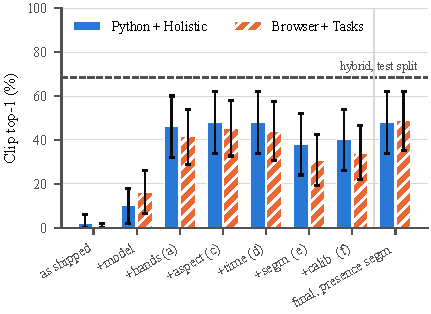
\includegraphics[width=\columnwidth]{figures/livegap}
\caption{Clip top-1 as the fixes are added one at a time, the final pipeline with presence
segmentation instead of the motion segmenter, and the hybrid's test top-1 (dashed); 95\%
bootstrap intervals over the \V{lg.clips} clips; browser bars are means over runs.}
\label{fig:livegap}
\end{figure}

Table~\ref{tab:livegap} and Figure~\ref{fig:livegap} give the ablation. The shipped build
recognized \V{lg.web.c0headbuild.top1}\% of the clips (top-3 \V{lg.web.c0headbuild.top3}\%). With
the hybrid and all fixes, clip top-1 reaches \V{lg.web.c6final.top1}\% \V{lg.web.c6final.top1ci}
in the browser and \V{lg.py.c6final.top1}\% \V{lg.py.c6final.top1ci} in Python (top-3
\V{lg.web.c6final.top3}\% and \V{lg.py.c6final.top3}\%). Measured from the hybrid with no fix,
this recovers \V{lg.web.recover}\% (browser) and \V{lg.py.recover}\% (Python) of the drop from its
\V{m.d.top1}\% test top-1, so most of the gap remains.

\paragraph{Hand slots had by far the largest effect.}
Adding the hand fix raised clip top-1 by \V{lg.py.c2hands.dtop1} points in Python and
\V{lg.web.c2hands.dtop1} in the browser (\V{lg.web.c2hands.dtop1better} clips better,
\V{lg.web.c2hands.dtop1worse} worse), and undoing it in the final pipeline cost
\V{lg.py.xhands.dtop1} and \V{lg.web.xhands.dtop1} points. In the pre-specified clip-level analysis
all four changes are significant after correction. With signs as the unit, they remain significant
in Python (Holm $p$ = \V{lg.py.c2hands.dtop1psign} and \V{lg.py.xhands.dtop1psign}) and for undoing
the fix in the browser (\V{lg.web.xhands.dtop1psign}), but not for adding it in the browser
(\V{lg.web.c2hands.dtop1psign}). Mirroring (b) was not a fault: detecting on the mirrored frame
changes little once hands are assigned by the pose (\V{lg.web.xmirrored.dtop1} points), and the
old label mapping fails with or without mirroring (\V{lg.web.xhands.top1}\% and
\V{lg.web.xmirroredlabel.top1}\%).

\paragraph{Aspect correction and segmentation: large but inconclusive.}
Removing all aspect correction from the final pipeline cost \V{lg.py.xaspectoff.dtop1} points in
Python and \V{lg.web.xaspectoff.dtop1} in the browser, and replacing presence segmentation by the
motion segmenter cost \V{lg.py.c5segmenter.dtop1} and \V{lg.web.c5segmenter.dtop1}; none of these
changes is significant after correction at either unit, so we treat them as inconclusive. The
shipped build's own aspect correction scored like the new rule (\V{lg.py.xaspectcalibrated.dtop1}
and \V{lg.web.xaspectcalibrated.dtop1} points), so the data show that some correction is needed,
not that the shipped one was wrong. The final pipeline with presence segmentation instead
(\cfg{x\_presence}) matches or beats every other configuration we measured,
\V{lg.py.xpresence.top1}\% in Python and \V{lg.web.xpresence.top1}\% in the browser. The motion segmenter's loss comes mostly from
whole signs it never segmented: \V{lg.py.c6final.noseg} clips in Python and
\V{lg.web.c6final.noseg} per browser run had no classified segment, against
\V{lg.py.xpresence.noseg} and \V{lg.web.xpresence.noseg} with presence segmentation, and the
segments it did cut were shorter (median \V{lg.web.c5segmenter.segms} against
\V{lg.web.c4time.segms} ms in the browser). Its thresholds assume the dataset's frames are
\V{seg.assumedfps} fps apart; if they are not, speeds are misestimated, which would produce missed
starts of this kind. We keep the pipeline as specified, because choosing a segmenter on these clips
would tune on the test.

\paragraph{The other changes.}
Swapping in the hybrid before any fix gained \V{lg.web.c1model.dtop1} points in the browser
(\V{lg.web.c1model.dtop1better} clips better, none worse; \V{lg.web.c1model.dtop1sig} at clip
level, not at sign level, Holm $p$ = \V{lg.web.c1model.dtop1psign}) and \V{lg.py.c1model.dtop1} in
Python, from a floor near zero. Resampling by time (d) cannot matter in Python, where the frame rate is constant and both clocks
give the same positions; in the browser it changed clip top-1 by \V{lg.web.c4time.dtop1} points.
Calibration (f) does not change a segment's top-1, though averaging over segments can move a clip's
(\V{lg.web.c6final.dtop1} points). Replacing the hybrid by the v1 CNN in the final pipeline cost
\V{lg.py.xv1model.dtop1} and \V{lg.web.xv1model.dtop1} points (\V{lg.web.xv1model.dtop1sig}), so
the hybrid's test-set advantage shows only weakly here.

\paragraph{What remains.}
The two pipelines differ by little: browser minus Python is \V{lg.pd.c6final.diff} points
\V{lg.pd.c6final.ci} for the final pipeline and \V{lg.pd.xpresence.diff} \V{lg.pd.xpresence.ci} with
presence segmentation (signs as the unit). The training tracker is therefore not what separates
these clips from the test split; the remaining gap lies in what both live pipelines share, above all
segmentation, or in the clips themselves (signer, camera, room and the signer's productions), which
this design cannot separate. \V{lg.failboth} of the \V{lg.signs} signs fail in every take in both
pipelines, and for \V{lg.sharedconf} the most frequent wrong guess is the same in both
(\V{lg.sharedconflist}; Table~\ref{tab:persign}).

\paragraph{Live abstention.}
On the live segments the calibration does not hold: the expected calibration error is
\V{lg.cal.web.ece} in the browser (\V{cal.test.ece1} on test). The validation threshold accepts
\V{lg.cal.web.cov}\% of segments at \V{lg.cal.web.sel}\% selective accuracy, a net score of
\V{lg.cal.web.net} against \V{cal.test.net} on test; it holds back \V{lg.cal.web.rejwrong}\% of
the wrong guesses but also \V{lg.cal.web.rejright}\% of the correct ones.
